\documentclass[lettersize,journal]{IEEEtran}
\usepackage{amsmath,amsfonts,amssymb}
\usepackage{algorithmic}
\usepackage{algorithm}
\usepackage{array}
\usepackage[caption=false,font=normalsize,labelfont=sf,textfont=sf]{subfig}
\usepackage{textcomp}
\usepackage{stfloats}
\usepackage{url}
\usepackage{verbatim}
\usepackage{graphicx}
\usepackage{cite}
\usepackage{multirow}
\usepackage{booktabs}
\usepackage{threeparttable}
\usepackage{enumitem}
\hyphenation{op-tical net-works semi-conduc-tor IEEE-Xplore}
% updated with editorial comments 8/9/2021


\usepackage{orcidlink}


\begin{document}

\title{Graph Learning for Topology-Adaptive Fast Frequency Response in Inverter-Based Microgrids}

% \author{IEEE Publication Technology,~\IEEEmembership{Staff,~IEEE,}
%         % <-this % stops a space
% \thanks{This paper was produced by the IEEE Publication Technology Group. They are in Piscataway, NJ.}% <-this % stops a space
% \thanks{Manuscript received April 19, 2021; revised August 16, 2021.}}

\author{Tran Kim Nhat, Nguyen Van Cuong\orcidlink{0000-0001-8877-7735},~\IEEEmembership{Graduate Student Member,~IEEE}, Nguyen Phi Long\orcidlink{0000-0002-3788-8731},~\IEEEmembership{Member,~IEEE}, and Laurent El Ghaoui\orcidlink{0000-0002-0499-5610}
	
%	\thanks{Manuscript received January 1, 20xx; revised xxxx xx, xxxx. \textit{(Corresponding author: Nguyen Phi Long)}. The authors acknowledge the financial support provided by the Vingroup Innovation Foundation (VINIF) under Project VINIF.2025.DA119.}
	
	\thanks{The authors acknowledge the financial support provided by the Vingroup Innovation Foundation (VINIF) under Project VINIF.2025.DA119. \textit{(Corresponding author: Nguyen Phi Long.)}}
		
	\thanks{T.K. Nhat, N.V. Cuong, N.P. Long, and Laurent El Ghaoui, are with Center for Environmental Intelligence and College of Engineering \& Computer Science, VinUniversity, Hanoi 100000, Vietnam (e-mail: nhat.tk@vinuni.edu.vn; 25cuong.nv@vinuni.edu.vn; long.np2@vinuni.edu.vn; laurent.eg@vinuni.edu.vn).}
	
	\thanks{N.V. Cuong and N.P. Long are also with School of Electrical and Electronic Engineering, Hanoi University of Industry, Hanoi 100000, Vietnam (e-mail: cuongnv@haui.edu.vn; long.nguyen04@haui.edu.vn).}
}



% The paper headers
% \markboth{Journal of \LaTeX\ Class Files,~Vol.~14, No.~8, August~2021}%
% {Shell \MakeLowercase{\textit{et al.}}: A Sample Article Using IEEEtran.cls for IEEE Journals}

%\IEEEpubid{0000--0000/00\$00.00~\copyright~2021 IEEE}
% Remember, if you use this you must call \IEEEpubidadjcol in the second
% column for its text to clear the IEEEpubid mark.

\maketitle

\begin{abstract}
High penetration of inverter-based resources (IBRs) in islanded microgrids reduces system inertia and makes fast frequency response (FFR) sensitive to feeder reconfiguration, which the fixed-gain, topology-blind droop loop cannot track. This paper proposes a topology-adaptive FFR controller that couples an inductive GraphSAGE encoder over the active feeder graph with a parameter-shared multi-agent proximal policy optimization (MAPPO) actor under centralized training with decentralized execution; each distributed energy resource jointly emits a fast active-power reference and a local droop gain. The training environment is a topology-dependent reduced state-space frequency model whose inter-unit coupling is reshaped by each reconfiguration through the Kron-reduced network Jacobian, and frequency security is enforced by a shared envelope a monotone-gain Lyapunov certificate and a closed-form nadir-projection layer applied identically to every controller. Trained on a single topology of a modified islanded IEEE 123-bus feeder and evaluated zero-shot on $24$ unseen reconfigurations, the proposed controller re-enters the ENTSO-E $\pm50$~mHz band $1.9$--$3.0\times$ faster than the learning baselines ($9$--$14$~s versus $17$--$43$~s) with a $20$--$72\times$ lower time-weighted error, and retains its post-event integral frequency error within $6\,\%$ of the training-feeder value across the hold-out the lowest unseen error of any controller, $53\,\%$ below the next-best learning baseline, whose errors grow by $112$--$421\,\%$. Against fixed droop it raises the severe-event nadir by up to $1.0$~Hz at the lowest per-event cost of the learning controllers ($1.73$--$1.78$~\texteuro).
\end{abstract}



\begin{IEEEkeywords}
Fast frequency response (FFR), islanded microgrids (IMGs), inverter-based resources (IBR), virtual power plant (VPP), GraphSAGE network, multi-agent reinforcement learning (MARL), proximal policy optimization (PPO)
\end{IEEEkeywords}

% =====================================================================
\section*{Nomenclature}
\begin{IEEEdescription}[\IEEEsetlabelwidth{$\Delta P_{\mathrm{ref}},\Delta P_{\mathrm{imb}}$}]
\item[$g,\,i,\,m,\,t$] Index of GFM unit, DER, agent, time step.
\item[$I,\,L$] Retained GFM buses; eliminated load buses.
\item[$\mathcal{A},\,\mathcal{Z}$] Set of GFL agents; set of VPP zones.
\item[$\mathcal{G}_t,\,\mathcal{N}(j)$] Active feeder graph; neighborhood of node $j$.
\item[$H_g,\,H_{\mathrm{sys}}$] GFM virtual inertia; aggregate system inertia.
\item[$D_g,\,n_g$] GFM damping coefficient; number of GFM units.
\item[$f_0,\,\omega_0$] Nominal frequency; $\omega_0=2\pi f_0$.
\item[$S_{\mathrm{base}},\,S_g$] System base power; rating of unit $g$.
\item[$P_{\mathrm{rated}},\,\Delta t$] DER rated power; fast control step.
\item[$K_{\min},K_{\max}$] Lower/upper droop-gain bound.
\item[$\delta$] Nadir-admissible COI band ($0.5$\,Hz).
\item[$\gamma,\,\lambda,\,\epsilon$] Discount; GAE factor; PPO clip range.
\item[$\Delta\omega_g,\Delta\delta_g$] Frequency/angle deviation of unit $g$ (vectors $\Delta\boldsymbol{\omega}$, $\Delta\boldsymbol{\delta}_{\mathrm{rel}}$).
\item[$x,\,u_t$] State vector; control input.
\item[$\Delta P_{\mathrm{set},g},\Delta P_{e,g}$] Power set point; electrical-power deviation.
\item[$\Delta P_{\mathrm{ref}},\Delta P_{\mathrm{imb}}$] Commanded reference; disturbance imbalance.
\item[$\Delta P^{\mathrm{ffr}}_{i,t},\,R^{\mathrm{ffr}}_{i,t}$] Incremental FFR power; deliverable reserve.
\item[$\mathrm{SoC}_t$] State of charge.
\item[$V_t,S_t,P_t,Q_t$] Voltage, loading, and line-flow profiles.
\item[$\Delta f_t,\,\dot f_t$] COI frequency deviation; RoCoF.
\item[$a_m,a^P_m,a^K_m$] Agent action; power and droop channels.
\item[$K_m$] Learned local droop gain of agent $m$.
\item[$H_j^{(k)}$] Embedding of node $j$ at GraphSAGE layer $k$.
\item[$r_t,\,\hat A_t,\,\rho_t$] Team reward; GAE advantage; PPO ratio.
\item[$A_f(\mathcal{G}_t,K_t)$] Topology-parameterized state matrix.
\item[$B_{\mathrm{ref}},B_{\mathrm{net}}$] Reference and located-disturbance input maps.
\item[$\tilde J_r,\,J_{(\cdot)}$] Kron-reduced power Jacobian and blocks.
\item[$D(K_t)$] Effective damping matrix.
\item[$W_{\mathrm{self}},W_{\mathrm{neigh}}$] Shared GraphSAGE aggregator weights.
\item[$V,\,M$] Lyapunov function; inertia matrix.
\end{IEEEdescription}

\section{Introduction}
% ==================================================================
\label{sec:intro}
% ==================================================================

\IEEEPARstart{T}{he} transition toward $100$\,\% inverter-based resources (IBRs) in islanded distribution feeders removes the synchronous inertia that has traditionally bounded the rate of change of frequency (RoCoF), pushing the post-disturbance frequency \emph{nadir} toward under-frequency load-shedding (UFLS) thresholds and, in severe cases, blackout~\cite{roy2022overview}. Secure operation therefore requires the inverter-interfaced distributed energy resources (DERs) battery energy storage (BESS), vehicle-to-grid (V2G) chargers, and distributed photovoltaics (DPV) to deliver \emph{fast frequency response} (FFR) on sub-second-to-second time scales, coordinated with the grid-forming (GFM) inverters that set the voltage and frequency reference~\cite{perez2023adaptive,salem2025gfmreview}. The scheme deployed today is the \emph{classical droop} controller, in which each DER injects a power increment proportional to the local frequency deviation,
\begin{equation}
\Delta P^{\mathrm{ffr}}_{i,t}=-K_i\,\Delta f_t,
\label{eq:classical_droop}
\end{equation}
with a fixed per-device gain~$K_i$. This loop has two structural limitations. \emph{First, the gain is fixed:} commissioned for the worst foreseeable event, it is under-utilized during mild disturbances and cannot amplify near UFLS or surrender headroom when storage energy is scarce~\cite{boutfarjoute2025fuzzy,kerdphol2017robust}. \emph{Second, the controller is topology-blind:} FFR deliverability is set jointly by the DER fleet and the active feeder graph, which distribution-system-operator (DSO) tie-switch reconfiguration and line contingencies continually reshape~\cite{mohyuddin2022dsovpp,jacob2024outage}, yet neither $K_i$ nor the state in~\eqref{eq:classical_droop} encodes the active graph.

Adaptive virtual-inertia and virtual-synchronous-generator (VSG) control improves RoCoF and nadir over fixed droop under time-varying generation, and field demonstrations confirm that GFM--VSG inverters can stabilize a 100\% IBR microgrid without rotating machines~\cite{hamanah2024robust}; these controllers, however, are re-tuned by small-signal analysis around a fixed feeder and operating point, treating topology variation as parametric uncertainty rather than a structural change of the graph. Multi-agent reinforcement learning (MARL) under centralized training with decentralized execution (CTDE) coordinates large DER populations for dispatch, voltage, and primary frequency control~\cite{dolatyabi2025happo,shi2025coordvpp,qiu2023hierarchical}, yet standard formulations rely on multi-layer-perceptron (MLP) encoders or transductive graph convolutions that embed a \emph{fixed} adjacency~\cite{wang2025mappo,wang2023graphppo,guo2024gcnnppo,guo2024ldlfc}, binding observations, message-passing neighborhoods, and policies to the training graph, and they expose either a power-reference \emph{or} a droop-gain action, rarely both~\cite{hu2022multitimescale}. Inductive graph neural networks such as GraphSAGE~\cite{hamilton2017graphsage} learn aggregator functions that generalize to unseen graphs and have been applied to topology-varying emergency control on transmission systems~\cite{pei2023graphsage,CHEN2023930}; to our knowledge, however, no prior study combines an inductive encoder, a per-DER joint power-reference/droop-gain action, and an islanded $100$\,\% IBR setting under a zero-shot topology hold-out. We accordingly disclaim novelty of GraphSAGE itself and of the GraphSAGE--RL combination~\cite{pei2023graphsage}; the contribution lies in the problem, the architecture, and the evaluation.

Three gaps persist. FFR deliverability is commonly modeled from the local energy state alone, ignoring the active graph and the resulting voltage and current envelopes. The power reference and the droop gain are never exposed to the policy jointly, so the controller can neither pre-position storage nor trade transient support against energy headroom in real time. And MARL FFR controllers are almost universally evaluated on their training topologies, leaving the zero-shot generalization gap on frequency-security metrics nadir, integral absolute error (IAE), RoCoF, and UFLS success rate unquantified.

This paper closes these gaps with three contributions.

\begin{enumerate}[leftmargin=*]
  \item \textbf{Topology-coupled deliverability and frequency model.} We cast the available FFR reserve and the effectiveness of a droop commitment as functions of the active feeder graph, bus voltages, and inverter loading, and evaluate the response through a topology-dependent reduced state-space model $\mathbf{A}_f(\mathcal{G}_t,\mathbf{K}_t)$ whose inter-GFM coupling is reshaped by each reconfiguration through the Kron-reduced network Jacobian removing the inconsistency of driving a topology-adaptive policy with a reconfiguration-invariant centre-of-inertia model.

  \item \textbf{GraphSAGE--MAPPO with a joint action and a safety envelope.} An inductive GraphSAGE encoder over the active graph feeds a parameter-shared MAPPO actor under CTDE that emits, per DER, a joint power-reference/droop-gain action $(a^{P}_{i,t},a^{K}_{i,t})$, replacing the fixed-gain droop loop. Frequency security is enforced as a shared safe-by-construction envelope: a monotone-gain parameterization with a Lyapunov certificate over the feasible topology set, backbone-governed RoCoF, and a closed-form nadir-projection layer.

  \item \textbf{Zero-shot topology hold-out on frequency-security metrics.} We train on a single feeder topology and evaluate zero-shot on $24$ disjoint unseen reconfigurations of a modified islanded IEEE 123-bus feeder, isolating the source of topology adaptation through an encoder-only ablation under an identical learning stack to our knowledge the first MARL FFR controller for islanded microgrids verified this way.
\end{enumerate}

The remainder of the paper is organized as follows. Section~\ref{sec:model} presents the islanded IBR microgrid, its component and topology-dependent frequency-dynamics models, and the three-layer DSO--VPP--DER execution architecture. Section~\ref{sec:method} casts real-time FFR as a cooperative Dec-POMDP and details the GraphSAGE--MAPPO controller and its safety envelope. Section~\ref{sec:casestudy} describes the test system, training, and hold-out protocol; Section~\ref{sec:results} reports the case studies; and Section~\ref{sec:conclusion} concludes.




\section{System Model and Problem Formulation}
\label{sec:model}
%                        
\subsection{Islanded 100\,\% Inverter-Based Microgrid and Component Models}
\label{sec:model:overview}
\subsubsection{Grid-Forming Backbone}
A backbone of $n_g$ grid-forming (GFM) inverters establishes the voltage and frequency references. Each unit $g$ emulates the swing dynamics of a synchronous machine through a virtual-inertia control loop \cite{hou2020adaptive,fathi2018extended},
\begin{align}
  2H_g\,\frac{d\Delta\omega_g}{dt}
    &= \Delta P_{\mathrm{set},g}-\Delta P_{e,g}-D_g\,\Delta\omega_g,
       \label{eq:vsg_swing}\\
  \frac{d\Delta\delta_g}{dt} &= \omega_0\,\Delta\omega_g,
       \label{eq:vsg_angle}
\end{align}
where $\Delta P_{e,g}$ is the network-imposed electrical-power deviation, introduced below, and the virtual inertia $H_g$ is a programmable control parameter rather than rotating mass \cite{10638828}. The backbone is heterogeneous: one unit is configured as a full virtual synchronous generator (VSG) carrying the largest virtual inertia, while the remaining $n_g-1$ units operate as droop grid-forming inverters with a lower inertia floor (per-unit values in Table~\ref{tab:system}). Two consequences follow: the immediate post-disturbance RoCoF equals $\Delta P_{\mathrm{imb}}/(2H_{\mathrm{sys}})$, fixed by the aggregate backbone inertia and not alterable by any downstream power command within the first step, while $D_g$ shapes the post-nadir settling. The backbone therefore governs RoCoF, while the grid-following fleet supplies additional post-disturbance damping.

\subsubsection{Grid-Following DER Fleet}
A fleet of $|\mathcal{A}|$ grid-following (GFL) DERs BESS, V2G chargers, and DPV injects active power and a learned droop term but does not emulate inertia. These are the controllable agents of the proposed method, modeled at the level of detail required by the one-second fast step $\Delta t$; the inner voltage and current loops settle far faster than $\Delta t$ and are represented by their first-order envelopes. A BESS agent is a state-of-charge (SoC) integrator with separate charge/discharge efficiencies, held within a physical SoC band; a V2G agent augments this recursion with connection availability, a discharge-enable SoC threshold, a usable-capacity cap, and a first-order response lag, and leaves the fleet at its departure step, so the controllable set is time-varying. DPV operates at maximum power point and provides curtailment-only (non-positive) regulation, treated as instantaneous at the fast step. The device recursions and the located-disturbance and discretization maps are collected in the supplementary material (Sec.~S-I).

\subsubsection{Deliverable FFR Reserve}
The reserve a DER can actually deliver is not a function of its energy state alone. In an islanded feeder it depends on the active topology and on the resulting voltage and current envelopes,
\begin{equation}
  R^{\mathrm{ffr}}_{i,t}
   = f\!\left(\mathcal{G}_t,\ \mathrm{SoC}_{i,t},\ V_t,\ S_t,\ P_t,\ Q_t\right).
  \label{eq:deliverability}
\end{equation}
A controller that ignores $\mathcal{G}_t$ commits a reserve that cannot be delivered under the realized topology, producing under-supply and larger frequency excursions. This relation motivates the topology-dependent frequency model developed next and is the physical basis of the first contribution.

%                        
\subsection{Topology-Dependent Frequency Model}
\label{sec:model:freqmodel}

The classical center-of-inertia (COI) model collapses the feeder to a single scalar swing equation and therefore cannot express how tie-switch reconfiguration or line contingencies redistribute the frequency response. We instead retain the inter-unit angle structure and let the active feeder graph enter the state matrix explicitly. The COI quantity is recovered only as a read-out.

\subsubsection{Reduced-Order State Space}
Collect the GFM deviations into the state $x=\big[\Delta\boldsymbol{\delta}_{\mathrm{rel}}\in\mathbb{R}^{n_g-1},\
\Delta\boldsymbol{\omega}\in\mathbb{R}^{n_g}\big]^{\!\top}$, the relative angles being referenced to the largest-rated GFM unit. Assembling \eqref{eq:vsg_swing}--\eqref{eq:vsg_angle} over the backbone gives the linear, topology-parameterized dynamics
\begin{equation}
  \frac{dx}{dt}
   = A_f(\mathcal{G}_t,K_t)\,x
     + B_{\mathrm{ref}}\,\Delta P_{\mathrm{ref}}
     + B_{\mathrm{net}}\,\Delta P_{\mathrm{imb}},
  \label{eq:statespace}
\end{equation}
with the block state matrix
\begin{equation}
  A_f(\mathcal{G}_t,K_t)=
  \begin{bmatrix}
     \mathbf{0} & \omega_0\,\mathbf{1}^{-1}\\[4pt]
     -\operatorname{diag}\!\big(\tfrac{1}{2H}\big)\,\tilde{J}_r(\mathcal{G}_t)
        & -\operatorname{diag}\!\big(\tfrac{1}{2H}\big)\,D(K_t)
  \end{bmatrix},
  \label{eq:af_matrix}
\end{equation}
where $\mathbf{1}^{-1}$ is the reference-subtraction (relative-angle) map and $D(K_t)=\operatorname{diag}(K_{\mathrm{eff},g})$ collects the effective damping set by the learned droop gains $K_t$.

\subsubsection{Topology Entry via Kron Reduction}
The active feeder graph $\mathcal{G}_t$ enters the state matrix through the Kron-reduced active-power Jacobian $\tilde{J}_r(\mathcal{G}_t)$, obtained by eliminating the passive buses of the energized feeder \cite{luo2014kronmicrogrid,ajala2023gfmreduction},

\begin{equation}
  \tilde{J}_r = J_{II}-J_{IL}\,J_{LL}^{-1}\,J_{LI}.
  \label{eq:kron}
\end{equation}
Tie-switch reconfiguration and line contingencies change the block partition in \eqref{eq:kron}, so each topology produces a distinct $\tilde{J}_r$ and hence a distinct synchronizing-torque coupling among the GFM units. The topology therefore acts through $\tilde{J}_r$ while the learned droop acts through $D(K_t)$; the block structure of $A_f$ makes both dependencies explicit, which the scalar COI model cannot.

\subsubsection{Located Disturbance Entry}
The imbalance $\Delta P_{\mathrm{imb}}$ is injected at the \emph{physical} feeder bus of the contingency, not spread uniformly across units, so the input matrix $B_{\mathrm{net}}(\mathcal{G}_t)$ is itself topology-dependent through the Kron transfer $J_L(\mathcal{G}_t)$ (derived in the supplementary material). A contingency electrically close to unit $g$ then loads $g$ more than distant units, and a reconfiguration that re-routes around $g$ redistributes that loading. The active graph $\mathcal{G}_t$ thus shapes not only the synchronizing coupling in $\tilde{J}_r$ but also \emph{where} the disturbance is felt; a controller blind to $\mathcal{G}_t$ can anticipate neither effect.

\subsubsection{Discretization, Read-Out, and Secondary Control}
Because $\Delta t=1$\,s is large relative to the inverter time constants, the model is discretized by zero-order hold to $(\Phi,\Gamma)$, evaluated by the augmented matrix exponential and cached per topology and droop-gain bin. The COI frequency is recovered as a rating-weighted read-out,
\begin{equation}
  \Delta f_t = f_0\,\frac{\sum_g S_g\,\Delta\omega_g}{\sum_g S_g},
  \qquad
  \dot f_t = \frac{\Delta f_t-\Delta f_{t-1}}{\Delta t},
  \label{eq:coi_readout}
\end{equation}
so the COI is an observable of the reduced dynamics rather than the state itself, and it is also the input to a slow integral secondary loop that removes the steady-state offset (supplementary material). The only lumped aggregate the model carries is the rating-weighted backbone inertia $H_{\mathrm{sys}}$; since $H_g$ is \emph{programmable virtual} inertia, $H_{\mathrm{sys}}$ is set by control rather than by physical machines. Unlike the single-COI swing model, the closed loop carries \emph{no} aggregate damping or droop constant: damping and droop enter per unit through $D(K_t)$, set by the backbone droop plus the learned grid-following droop. The numerical value of $H_{\mathrm{sys}}$ is reported in Section~\ref{sec:casestudy}.

\subsubsection{Frequency-Security Read-Out and Timescale}
Frequency security is assessed on the COI read-out \eqref{eq:coi_readout}: at the one-second FFR control step the COI is the resolvable system-frequency observable, in line with the standard reduced-order system-frequency-response (SFR) modelling of the FFR literature \cite{anderson1990sfr}. The relative-angle block of \eqref{eq:af_matrix} lets individual units' frequencies differ \emph{during} the transient, but these inter-machine deviations are a sub-second phenomenon below the control step; we report them only as a transient spatial diagnostic (worst-unit excursion, supplementary material), not as a headline metric. Crucially, topology shapes the \emph{COI} response itself, not merely its read-out: both the synchronizing coupling $\tilde{J}_r(\mathcal{G}_t)$ and the located forcing $B_{\mathrm{net}}(\mathcal{G}_t)$ are topology-dependent, so reconfiguration changes the equivalent inertia and damping seen by the COI and, through the deliverability relation, which committed reserve is actually deliverable   the channels a topology-aware controller must exploit \cite{luo2014kronmicrogrid,ajala2023gfmreduction}.

A modal property of \eqref{eq:af_matrix} underpins this read-out choice. Because the rows of $\tilde{J}_r$ sum to approximately zero (angle-reference invariance; only the retained resistive losses break the identity), the rating-weighted COI decouples from the synchronizing block and is governed by a single real mode, $\lambda_{\mathrm{COI}}\approx-\sum_g K_{\mathrm{eff},g}\big/\sum_g 2H_g$, while the inter-machine swing pairs of the stiff, Kron-reduced distribution feeder lie at tens to hundreds of hertz and cancel in the rating-weighted sum. The COI trajectory is therefore quasi-first-order   there is no governor-style oscillatory tail, unlike synchronous-machine SFR models   and the learned action shapes the recovery exclusively through the damping channel $D(K_t)$ and the reference channel $\Delta P_{\mathrm{ref}}$; the modal analysis is given in the supplementary material (Sec.~S-II).



%                        
\subsection{Three-Layer Economic VPP--DSO Coordination}
\label{sec:model:layers}

The DER fleet is organized for market participation by partitioning the feeder into $|\mathcal{Z}|$ virtual power plant (VPP) zones with agent sets $\mathcal{A}_z$, $\mathcal{A}=\bigcup_{z\in\mathcal{Z}}\mathcal{A}_z$. The real-time controller acts inside a three-layer coordination that separates grid feasibility, market-facing aggregation, and fast execution (Fig.~\ref{fig:architecture}): the DSO clears a second-order-cone OPF with feeder reconfiguration and posts the DLMP and the active topology \cite{bai2018dlmp,basdomenech2024dlmp}; the VPP aggregator returns a deliverable energy-and-reserve offer from a Wasserstein distributionally-robust bid under price and renewable uncertainty \cite{liu2021wdrovpp,arrigo2021wdroreserve}; and the proposed controller executes the fast active-power and droop commands against these signals as a \emph{price taker}, the standard hierarchical structure shown to coincide with centralized clearing \cite{huang2015dlmp,li2014dlmp}. Real-time delivery is not fed back to re-clear the upper layers within the horizon (no price impact); closed-loop coupling and price-making bids \cite{baringo2021pricemaker} are left to future work.

\begin{figure}[!t]
\centering
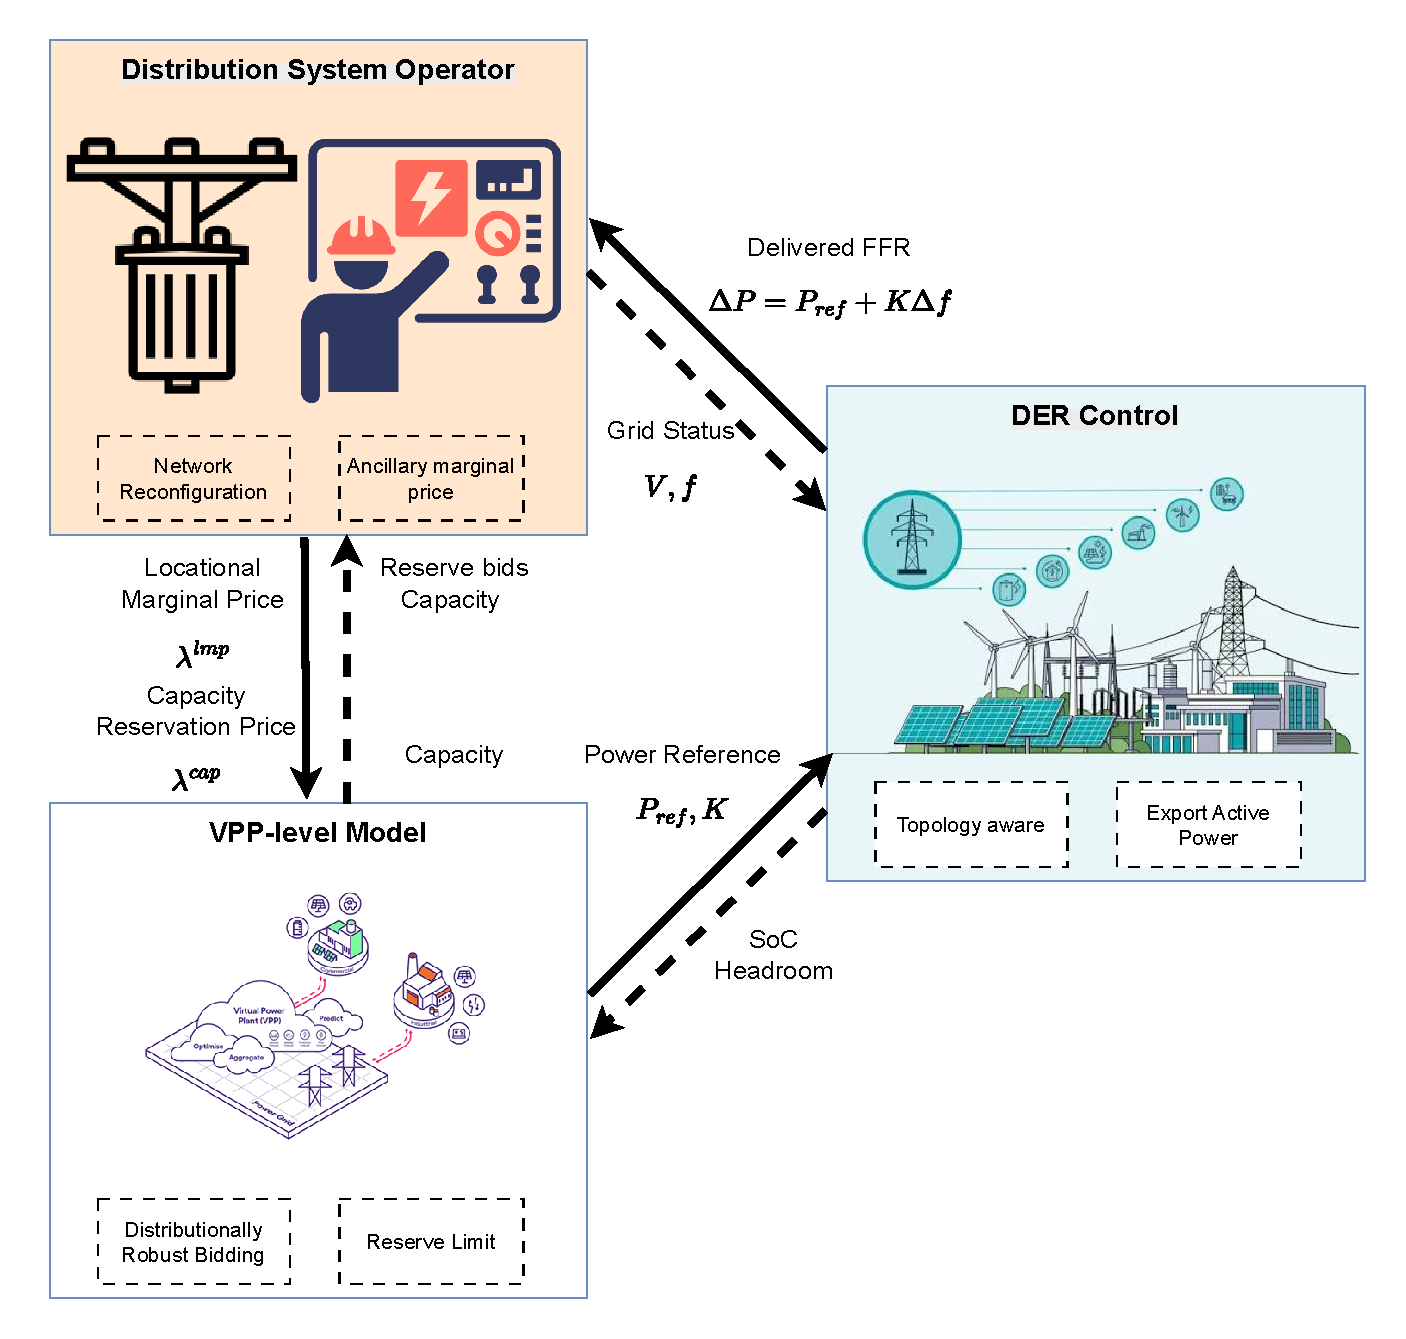
\includegraphics[width=0.92\linewidth]{img/architecture_3layer.png}
\caption{Three-layer DSO-VPP-DER coordination: the DSO posts DLMP and the active topology, the VPP aggregator returns a robust energy-and-reserve offer, and the proposed Layer-2 controller dispatches the DER fleet in real time as a price taker.}
\label{fig:architecture}
\end{figure}

% =====================================================================
\section{Proposed GraphSAGE-MAPPO Controller}
\label{sec:method}

\begin{figure}[!t]
\centering
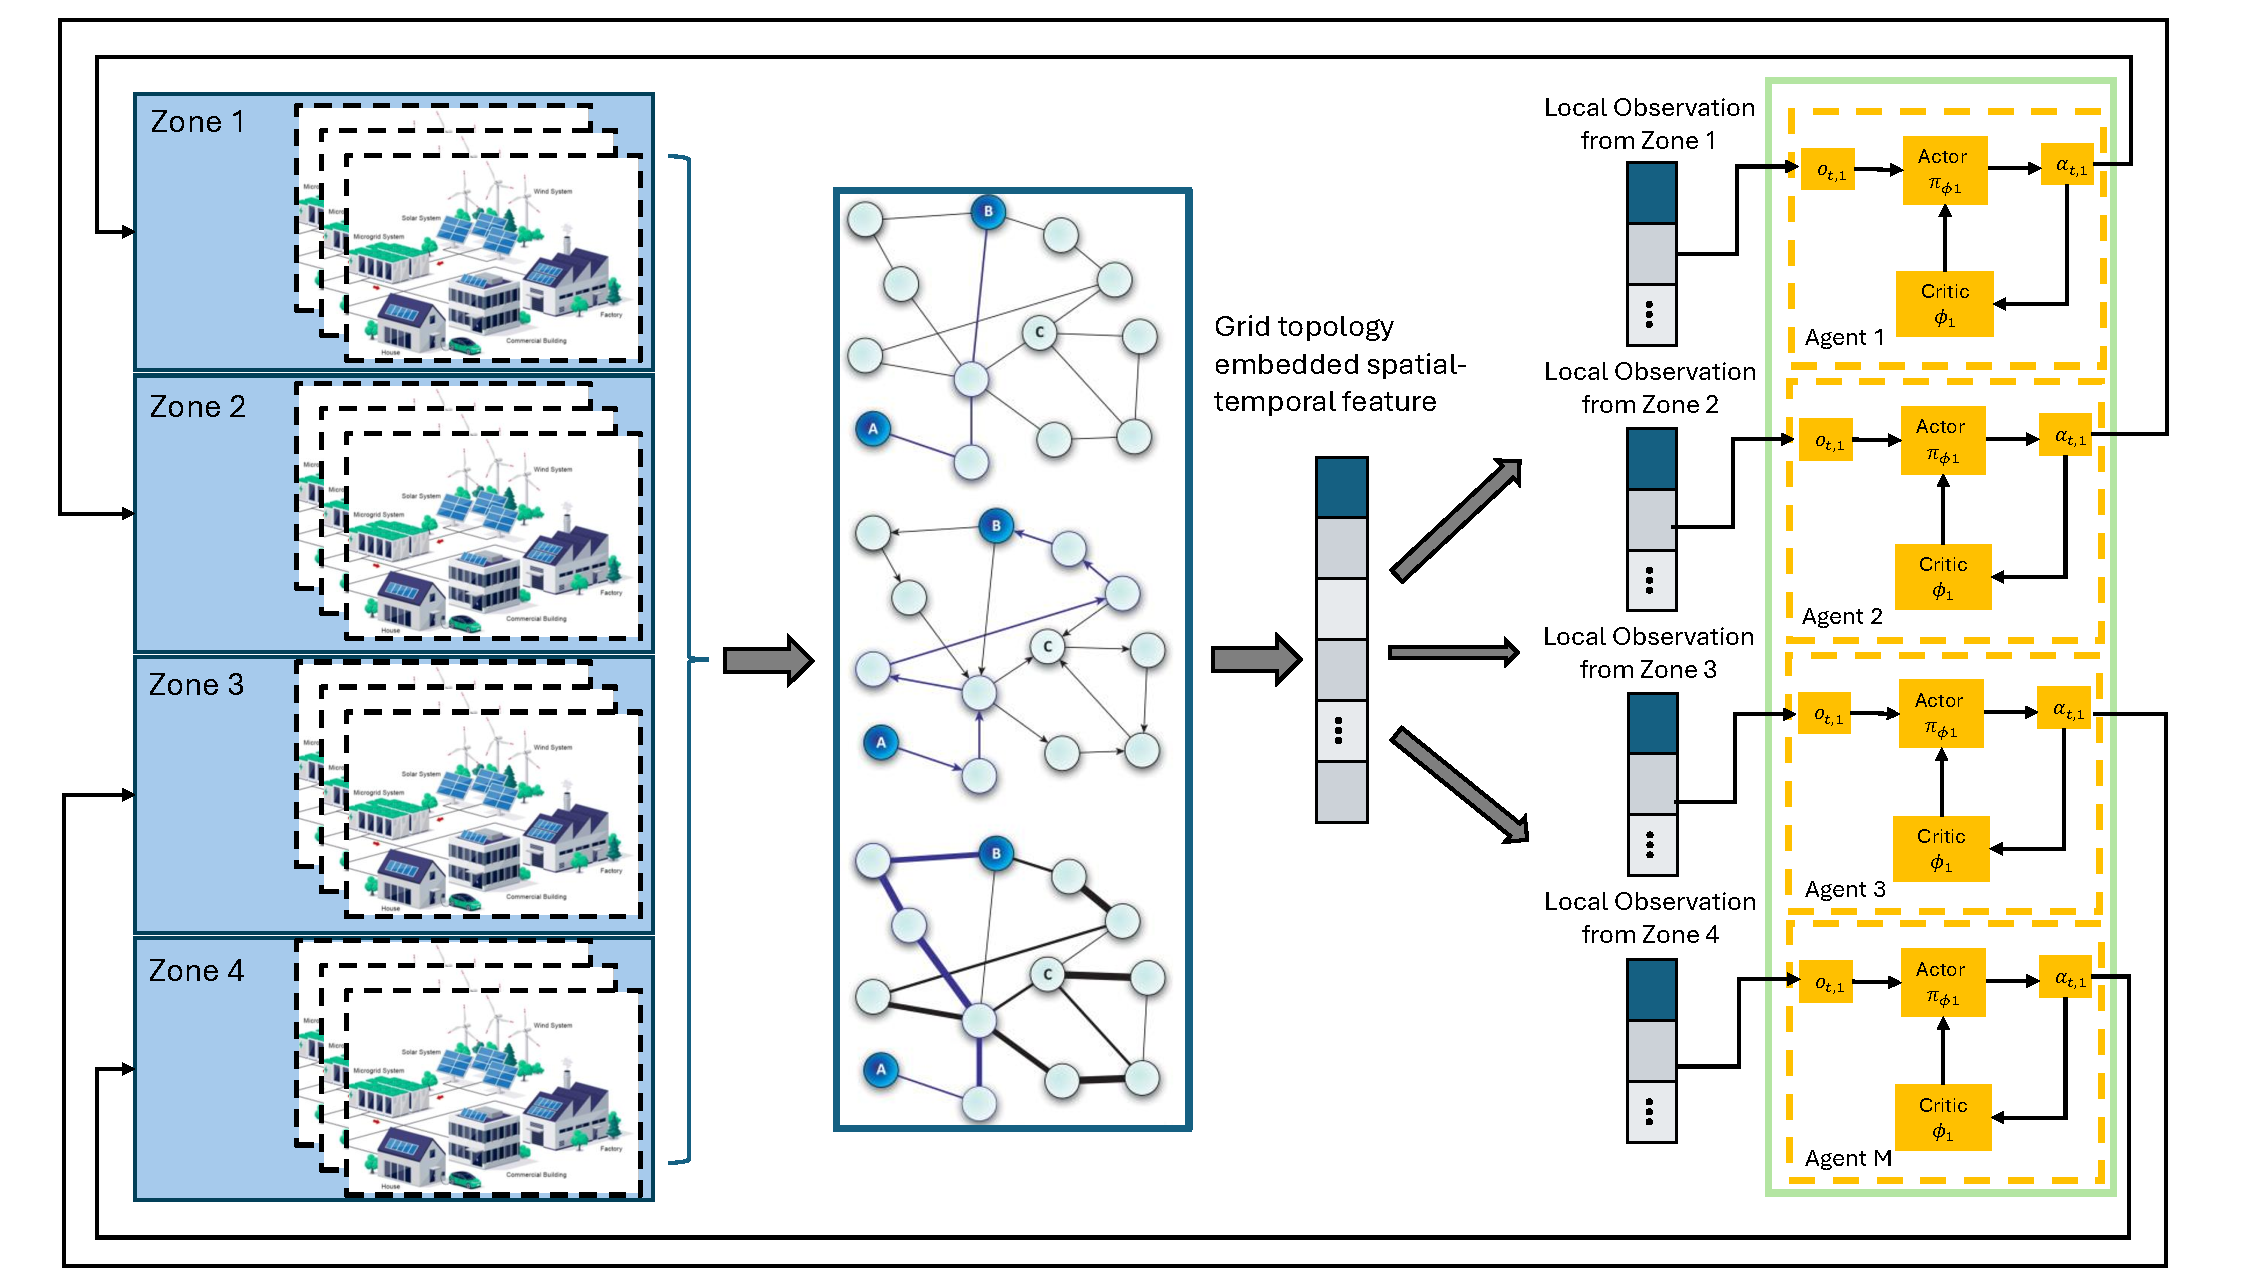
\includegraphics[width=1\linewidth]{img/GraphSAGE-MAPPOargi.pdf}
\caption{Proposed GraphSAGE-MAPPO controller.}
\label{fig:method_arch}
\end{figure}
%                        
\subsection{FFR as a Cooperative Dec-POMDP}
\label{sec:method:mdp}

The overall controller architecture is shown in Fig.~\ref{fig:method_arch}. The 41 GFL agents observe only local and neighborhood information, so the FFR task is a decentralized partially observable Markov decision process (Dec-POMDP) $\langle\mathcal{A},\mathcal{S},\{O_m\},\{U_m\},P,r,\gamma\rangle$ solved under centralized training with decentralized execution (CTDE). The fast step is $\Delta t=1$\,s with 300 steps per episode.

\subsubsection{Observation}
Each agent $m$ observes a 16-dimensional local vector comprising the local frequency deviation and RoCoF from the COI read-out, net power, SoC and dischargeable-energy headroom, the zonal locational marginal price, a four-way device-type one-hot encoding, VPP membership, the previous droop gain and power reference, SoC violation flags, a persistence power forecast, and a departure proxy. The local vectors are placed on the 123-bus graph at their host buses and augmented with four per-bus grid-background features (active and reactive load, voltage magnitude, and agent density), giving the full feeder observation $\mathit{obs}_{\mathrm{full}}\in\mathbb{R}^{123\times20}$.

\subsubsection{Action}
Each agent emits a two-dimensional action $a_m=[a^P_m,\,a^K_m]\in[-1,1]^2$ that jointly sets a fast active-power reference and a local droop gain, replacing the fixed-gain response $\Delta P^{\mathrm{ffr}}_{i,t}=-K_i\,\Delta f_t$ of the classical loop with a learned, state-conditioned one,
\begin{align}
  \Delta P_m &= a^P_m\cdot 0.1\,P_{\mathrm{rated},m},
  \label{eq:action_power}\\
  K_m &= K_{\min,m}+\tfrac{1}{2}\big(1+a^K_m\big)\big(K_{\max,m}-K_{\min,m}\big).
  \label{eq:action_droop}
\end{align}
The two channels combine into the realized per-DER injection
\begin{equation}
  \Delta P^{\mathrm{ffr}}_{m,t} \;=\; \Delta P_m \;-\; K_m\,\Delta f_t,
  \label{eq:dual_law}
\end{equation}
a feed-forward reference plus a learned proportional (droop) feedback on the COI read-out; the classical loop \eqref{eq:classical_droop} is recovered as the special case $\Delta P_m=0$ with $K_m$ fixed. The power channel spans up to $\pm10\,\%$ of rated power (clipped to the device rating and SoC headroom, slew-limited at $0.2$/step); the droop channel spans $[K_{\min,m},K_{\max,m}]$ with $K_{\min,m}=0$ and per-type ceilings listed in Table~\ref{tab:system}. A droop gain is enabled only when $\mathrm{SoC}_m$ lies in the FFR-eligibility band, nested inside the physical band (Table~\ref{tab:system}); otherwise $K_m=0$. The per-DER commands aggregate to each host GFM unit   the reference channel in per unit on $S_{\mathrm{base}}$ and the droop channel as an additive contribution to the swing damping $D(K_t)$ after a MW/Hz-to-per-unit conversion   as detailed in the supplementary material (Sec.~S-I). Exposing $a^P_m$ and $a^K_m$ jointly lets the policy pre-position storage ahead of an anticipated FFR call and trade transient performance against service-quality constraints, which neither a power-only nor a droop-only formulation can do.
\subsubsection{Reward}
A single team reward couples frequency security, control effort, and service quality,

\begin{equation}
  r_t = r^{\Delta f}_t + r^{\mathrm{nadir}}_t + r^{\mathrm{viol}}_t
        + r^{\mathrm{ffr}}_t + r^{\mathrm{eff}}_t + r^{\mathrm{soc}}_t
        + r^{\mathrm{mkt}}_t + r^{\mathrm{commit}}_t,
  \label{eq:reward}
\end{equation}

where the frequency, nadir, and violation terms penalize the COI deviation from $f_0$ and its excursions beyond the safe band the same security target used for evaluation and applied identically to every controller, including the baselines the FFR-bonus term rewards staying within it, and the effort, SoC, market, and commitment terms regularize the action, penalize SoC violation, credit market revenue, and discourage abrupt gain changes. Error terms are normalized to $[0,1]$ against event-scaled references and combined by fixed weights; the explicit forms, deadbands, references, and weights of every term are given in the supplementary material (Sec.~S-V). The RoCoF term is disabled because peak RoCoF is governed by the GFM backbone rather than by the GFL action (Section~\ref{sec:method:safety}). The reward is passed through a running normalizer ($\gamma=0.99$, clipped at $\pm10$).

%                        
\subsection{Multi-Agent PPO under CTDE}
\label{sec:method:mappo}

The controller is trained with multi-agent proximal policy optimization (MAPPO) \cite{yu2022mappoeffective,schulman2017ppo} under CTDE: a centralized critic uses global information during training, while each agent executes from its local observation alone at run time. Both the actor and the critic operate on the per-agent embeddings produced by the encoder of Section~\ref{sec:method:graphsage}.

\emph{Actor.} A single parameter-shared diagonal-Gaussian policy maps each agent embedding through a two-layer perceptron to the mean and log-standard deviation of the two-dimensional action, with a bounded mean $\mu=0.75\tanh(\cdot)$ and $\sigma=\operatorname{softplus}(\cdot)+0.05$. Parameter sharing keeps the policy size independent of $|\mathcal{A}|$ and permits a varying agent count across topologies.

\emph{Critic.} A centralized critic concatenates each agent embedding with a global context formed by mean- and max-pooling over all agents and returns a per-agent value. The per-agent value retains credit information for each DER while the pooled context supplies the system-level signal needed for cooperative coordination.

\emph{Update.} Advantages are estimated by generalized advantage estimation ($\gamma=0.99$, $\lambda=0.95$) from the shared team reward
\eqref{eq:reward}, and the policy is updated by the clipped PPO surrogate with ratio $\rho_t$ and clip range $\epsilon=0.2$~\cite{schulman2017ppo} (supplementary material, Sec.~S-III). The total loss adds a value-regression term (coefficient $0.5$) and an entropy bonus annealed across the training curriculum.

%                        
\subsection{Inductive GraphSAGE Encoder}
\label{sec:method:graphsage}

The encoder is the component that makes the controller transferable to unseen feeder configurations. We use an inductive GraphSAGE encoder
\cite{hamilton2017graphsage}, which learns aggregator \emph{functions} over node neighborhoods rather than a fixed per-node embedding. For node $j$ at layer $k$,
\begin{equation}
  H_j^{(k)}
   = \sigma\!\Big(W_{\mathrm{self}}\,H_j^{(k-1)}
     + W_{\mathrm{neigh}}\!\cdot\!
       \operatorname{mean}_{u\in\mathcal{N}(j)} H_u^{(k-1)}\Big),
  \label{eq:graphsage}
\end{equation}
where $H_j^{(0)}$ is the per-bus observation and the aggregator weights are shared across all nodes and topologies. We use two layers, mapping the 20-dimensional input to a 128-dimensional hidden layer with ReLU and then to a 128-dimensional embedding.

\emph{Why inductive enables zero-shot transfer.} The edge index of $\mathcal{N}(j)$ in \eqref{eq:graphsage} is rebuilt at every step from the active graph $\mathcal{G}_t$; because the learned weights are properties of the aggregator rather than of any specific adjacency, reconfiguration changes which neighbors are aggregated but not the function that aggregates them. Transductive graph-convolution encoders, whose spectral filters are tied to a fixed adjacency, must instead be retrained when the graph changes; the inductive construction lets a single controller satisfy the topology-coupled deliverability relation without per-topology retraining.

\emph{Embedding extraction.} After two aggregation passes over the 123-bus graph, the embeddings at the 41 DER host buses are extracted and passed to the actor and the centralized critic. Both heads therefore reason over a representation that already encodes the neighborhood structure of the realized feeder.

%                        
\subsection{Shared Safety Envelope}
\label{sec:method:safety}

Frequency security is enforced by an envelope that is a property of the environment, not of any particular controller; the proposed policy and every baseline act inside the same envelope. The comparison therefore isolates performance and generalization within the safe set, not safety itself. The envelope rests on four mechanisms.

\emph{Stability by construction.} The map \eqref{eq:action_droop} with $K_{\min}=0$ keeps the droop gains non-negative, so the damping matrix
$D(K_t)=\operatorname{diag}(K_t)\succeq 0$ and the realized droop $-K_m\Delta f_t$ is monotone non-increasing in frequency \cite{feng2022stabilityrl,alduaij2025partialmonotone}.

\emph{Lyapunov certificate.} For the swing energy $V=\tfrac12\Delta\boldsymbol{\omega}^{\!\top}M\Delta\boldsymbol{\omega}+\tfrac12\Delta\boldsymbol{\delta}_{\mathrm{rel}}^{\!\top}\tilde{J}_r\Delta\boldsymbol{\delta}_{\mathrm{rel}}$, the derivative along the closed-loop dynamics is $\dot V=-\Delta\boldsymbol{\omega}^{\!\top}D(K_t)\Delta\boldsymbol{\omega}\le0$.
Since $A_f$ is affine in $K_t$ through $D(K_t)$, the vertices of the droop-gain box are extremal and a finite vertex check certifies Hurwitz stability over the full topology-by-gain set; the derivation, together with a switching (average dwell-time) certificate, is given in the supplementary material (Sec.~S-II).

\emph{RoCoF by system design.} The peak RoCoF satisfies $\dot f=\Delta P_{\mathrm{imb}}/(2H_{\mathrm{backbone}})$ and is set by the GFM backbone inertia, not by the GFL action in the first step \cite{kenyon2021gfmfreqorder}. The RoCoF reward term is consequently disabled in \eqref{eq:reward}.

\emph{Nadir projection.} A closed-form minimal-perturbation projection of $\Delta P_{\mathrm{ref}}$ keeps the predicted next-step COI deviation within $[-\delta,+\delta]$ ($\delta=0.5$\,Hz), using an affine predictor that mirrors the discretized dynamics and the located-disturbance forcing of the supplementary material. A single linear constraint gives a closed form with no quadratic program \cite{tabas2021safefilter}; the affine predictor and the projection formula are derived in the supplementary material (Sec.~S-IV). The guard acts on the COI because that is the resolvable system-frequency observable at the control step and the quantity the controller is rewarded and evaluated on.

% =====================================================================
\section{Case Study}
\label{sec:casestudy}



%
\subsection{Test System and Scenarios}
\label{sec:casestudy:system}
\label{sec:casestudy:scenarios}

The controller is evaluated on a modified IEEE 123-bus distribution feeder operated as a 100\,\% inverter-based islanded microgrid (Fig.~\ref{fig:topology}); system and device parameters are given in Table~\ref{tab:system} and the frequency-security thresholds, taken from the ENTSO-E network codes and IEEE standards, in Table~\ref{tab:fsec_standards}.


\begin{figure}[!t]
\centering
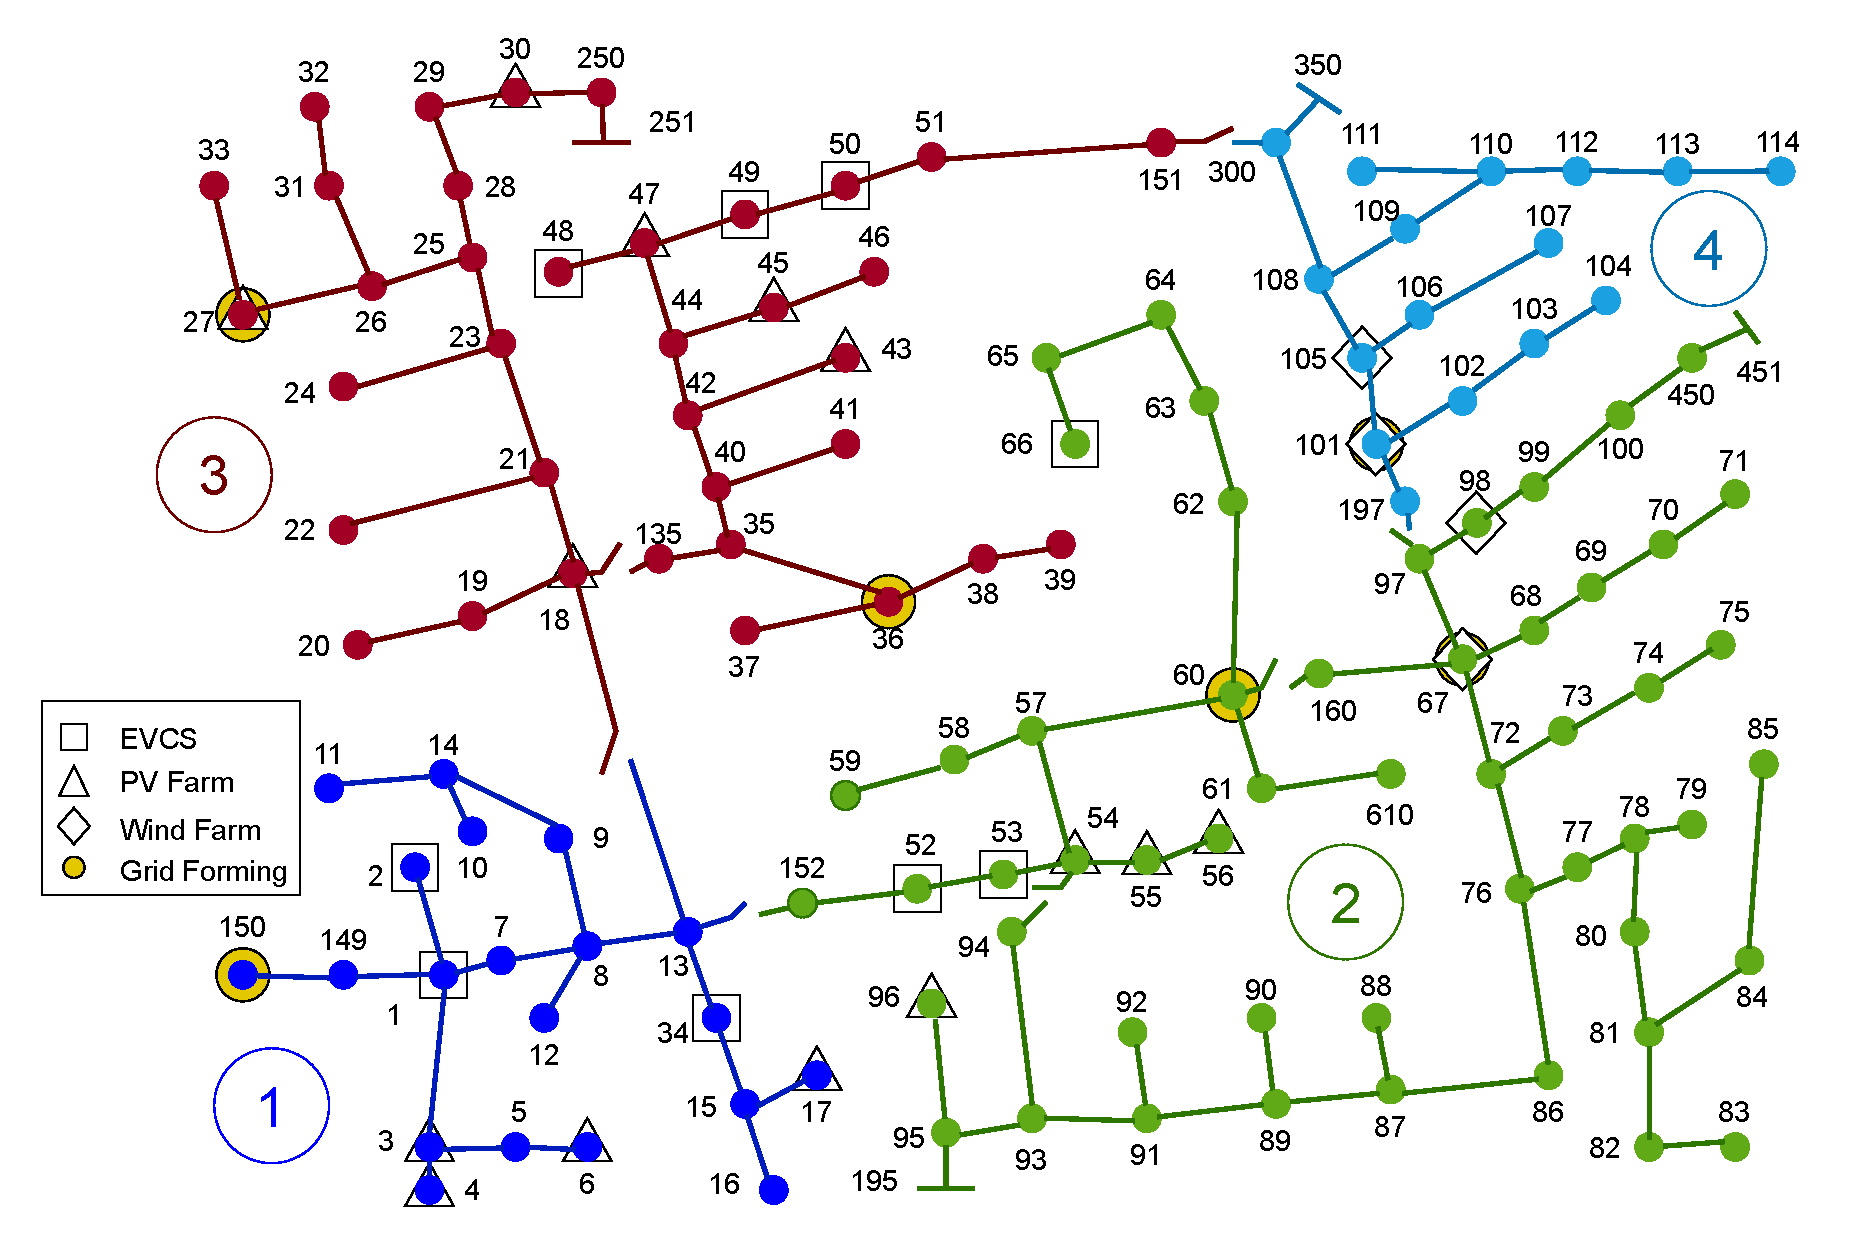
\includegraphics[width=0.95\linewidth]{img/Topology.pdf}
\caption{Islanded IEEE 123-bus feeder with VPP zones.}
\label{fig:topology}
\end{figure}


\begin{table}[!h]
\caption{System and device parameters.}
\label{tab:system}
\centering
\footnotesize
\resizebox{\linewidth}{!}{
\begin{tabular}{lll}
\toprule
Quantity & Symbol & Value \\
\midrule
Base power, frequency & $S_{\mathrm{base}}, f_0$ & $15.7$\,MW, $50$\,Hz \\
GFM backbone (VSG / droop) & $n_g, H_g$ & $6$ ($2.0$\,s / $0.5$\,s) \\
Aggregate system inertia & $H_{\mathrm{sys}}$ & $1.34$\,s \\
GFL agents, VPP zones & $|\mathcal{A}|, |\mathcal{Z}|$ & 41 agents, 34 zones \\
Droop ceiling (BESS/V2G/DPV) & $K_{\max}$ & $0.30$ / $0.20$ / $0.15 \cdot P_{\mathrm{rated}}$ \\
SoC band (Physical / FFR) &   & $[0.20, 0.90]$ / $[0.25, 0.85]$ \\
Efficiency, V2G response lag & $\eta, T_{\mathrm{v2g}}$ & $0.95$, $0.3$\,s \\
Time step, Episode length & $\Delta t$ & $1$\,s / $300$ steps \\
\bottomrule
\end{tabular}
}
\end{table}

\begin{table}[!t]
\caption{Frequency-security thresholds~\cite{entsoe_sogl_2017}.}
\label{tab:fsec_standards}
\centering
% \resizebox{\linewidth}{!}{
\begin{tabular}{ll}
\toprule
Quantity & Value\\
\midrule
UFLS Stage 1 trip       & $49.0$~Hz       \\
Operator alarm / FFR target & $49.5$~Hz   \\
UFLS Stage 1 delay      & $300$~ms        \\
RoCoF ride-through      & $2.0$~Hz/s      \\
FCR full activation     & $\pm 200$~mHz   \\
Standard freq.\ range (settling band) & $\pm 50$~mHz \\
\bottomrule
\end{tabular}
% }
\end{table}
The controller is exercised with four disturbance classes load step, generation trip, line trip, and high-renewable surge scaled as a fraction of $S_{\mathrm{base}}$ (Table~\ref{tab:scenarios}). Topology generalization is assessed under a strict zero-shot protocol: the controller is trained on a \emph{single} fixed feeder topology $G_0$ and evaluated, with no retraining or adaptation, on $24$ distinct reconfigurations $\mathcal{G}_{\mathrm{test}}=\{G_1,\dots,G_{24}\}$, $G_0\notin\mathcal{G}_{\mathrm{test}}$, generated from $G_0$ by tie-switch operations and $N{-}1$ line contingencies. Since radial reconfiguration changes only a bounded fraction of edges (Jaccard edge distance up to $\approx\!0.18$), the protocol stresses structural generalization within the reachable configuration space rather than transfer to arbitrary graphs.

\begin{table}[!t]
\caption{Contingency scenarios.}
\label{tab:scenarios}
\centering
\footnotesize
\resizebox{\linewidth}{!}{
\begin{tabular}{llccc}
\toprule
Sc. & Event       & $\Delta P$ (MW) & \% $S_{\mathrm{base}}$ & Purpose \\
\midrule
S1  & load step             & +2.5 & 16 & moderate          \\
S2  & generation trip       & -3.9 & 25 & severe under-freq. \\
S3  & line trip             &  2.4 & 15 & topology mutation  \\
S4  & high-renewable surge  & +4.7 & 30 & over-freq. stress  \\
\bottomrule
\end{tabular}
}
\end{table}

%
\subsection{Baselines and Training Protocol}
\label{sec:casestudy:baselines}
\label{sec:casestudy:training}

The proposed controller is compared against five baselines (Table~\ref{tab:methods}). All learning baselines run in the identical environment, observation, dual action, reward, and shared safety envelope of Sections~\ref{sec:model}--\ref{sec:method}; only the encoder or learning algorithm differs, so the comparison isolates each architectural component rather than safety itself. MLP-MAPPO isolates the value of graph message-passing; GCNN-PPO is a transductive, single-centralized state-of-the-art reference, differing in both encoder and agent structure rather than serving as a clean inductive-versus-transductive control.


\begin{table}[!h]
\caption{Baselines and the component each isolates.}
\label{tab:methods}
\centering
\footnotesize
\resizebox{\linewidth}{!}{
\begin{tabular}{lllll}
\toprule
\# & Method & Encoder & RL algorithm & Multi-agent \\
\midrule
1 & GraphSAGE-MAPPO (\emph{ours}) & GraphSAGE   & PPO  & MAPPO (CTDE)         \\
2 & MLP-MAPPO (ablation)          & MLP         & PPO  & MAPPO (CTDE)         \\
3 & GCNN-PPO~\cite{guo2024gcnnppo}& Spectral GCN& PPO  & Single centralized   \\
4 & MATD3~\cite{li2025matd3}      & MLP         & TD3  & CTDE                 \\
5 & Fixed droop                   &           &    &                    \\
6 & No FFR                        &           &    &                    \\
\bottomrule
\end{tabular}
}
\end{table}
Training uses a six-phase disturbance curriculum of $6000$ episodes that escalates event magnitude and probability from load-only events to the full $N{-}1$ mix at $40\,\%$ contingency magnitude; the per-phase schedule (episodes, event mix, magnitude, learning-rate and entropy factors) is tabulated in the supplementary material (Sec.~S-VI). Hyperparameters are selected by asynchronous successive halving (ASHA) on the evaluation IAE of the training feeder (12 sampled configurations, elimination factor $\eta=3$, stage budgets of $25/75/225$ episodes, multi-seed re-scoring at promotion; Sec.~S-VI), with the selected configuration in Table~\ref{tab:hyperparams} shared by every learning baseline   identical capacity, optimizer, curriculum, and training budget   so the proposed method enjoys no capacity or schedule advantage, and each method is reported at its converged performance.

\begin{table}[t]
  \centering
  \caption{Hyperparameters (ASHA-tuned; shared by all learning methods).}
  \label{tab:hyperparams}
  \begin{tabular}{lll}
    \hline
    Hyperparameter & Symbol & Value\\
    \hline
    Learning rate (phase-scheduled) &     & $3.1\times10^{-5}\rightarrow8\times10^{-6}$\\
    Discount / GAE         & $\gamma,\lambda$ & $0.99$, $0.95$\\
    PPO clip               & $\epsilon$     & $0.2$\\
    Entropy coefficient    &              & $5\times10^{-3}\rightarrow0$\\
    Embedding / hidden dim &              & $128$\,/\,$128$\\
    GraphSAGE layers       &              & $2$\\
    Update epochs / minibatch &           & $4$\,/\,$16$\\
    Curriculum length      &              & $6000$ episodes / $6$ phases\\
    \hline
  \end{tabular}
\end{table}

%
\subsection{Evaluation Protocol}
\label{sec:casestudy:metrics}

Performance is reported on three metric groups: frequency security (nadir, maximum RoCoF, IAE, settling time, FFR success rate), service and economics (committed reserve, energy-plus-capacity revenue), and topology generalization (training-to-unseen IAE gap and its spread). The frequency-security metrics are defined on the COI deviation $\Delta f(t)$ with event time $t_e$: the post-event integral error is windowed,
\begin{equation}
  \mathrm{IAE}_{\mathrm{post}}=\!\int_{t_e}^{t_e+T_w}\!\big|\Delta f(t)\big|\,dt,\qquad T_w=50~\mathrm{s},
  \label{eq:iae_post}
\end{equation}
complemented by the unwindowed $\mathrm{IAE}_{\mathrm{tot}}$ and the time-weighted $\mathrm{ITAE}=\int_{t_e}^{T}(t-t_e)\,|\Delta f|\,dt$, which expose post-window limit-cycle behavior that \eqref{eq:iae_post} cannot. The settling time is the first instant after which $|\Delta f|$ remains within $\pm50$~mHz   the ENTSO-E SO~GL standard frequency range (Table~\ref{tab:fsec_standards}). FFR success requires that no continuous excursion below the $49.5$~Hz alarm persists longer than the $300$~ms UFLS Stage-1 relay delay, checked on the $0.1$~s sub-step trace; formal definitions and the sub-step trace protocol are collected in the supplementary material (Sec.~S-VII). Each learning controller is evaluated zero-shot on the same $24$ unseen reconfigurations, and each per-topology value averages repeated episodes with randomized operating points and event timing. Table entries report the mean across held-out topologies with a $95\,\%$ confidence interval; the difference between the proposed controller and the next-best method on IAE and nadir is assessed by a paired Wilcoxon signed-rank test, and the proposed controller is trained from three independent random seeds, with consistent topology-generalization results across all three.



\section{Results and Discussion}
\label{sec:results}

All results below are computed from a single frozen evaluation of the converged controllers ($20$ episodes per scenario--method pair, metric definitions of Sec.~S-VII). Fig.~\ref{fig:radar_overview} summarizes the evaluation: for each contingency the six controllers are scored on five axes post-event IAE, nadir (or zenith) margin, settling speed, reliable reserve delivery, and topology robustness each oriented so that larger is better, grounded at zero, and normalized by the best in-group value. Two facts organize the results. First, the shared safety envelope holds the post-event nadir at the $49.5$~Hz alarm for \emph{every} learning controller, so all four achieve a unit FFR success rate while the two non-learning controls breach the alarm; safety is therefore common to the comparison, and the discriminators are integral error, settling speed, run-to-run consistency, and topology robustness. Second, on these discriminators the proposed controller encloses the largest area in all four contingencies.
 
\begin{figure*}[!t]
\centering
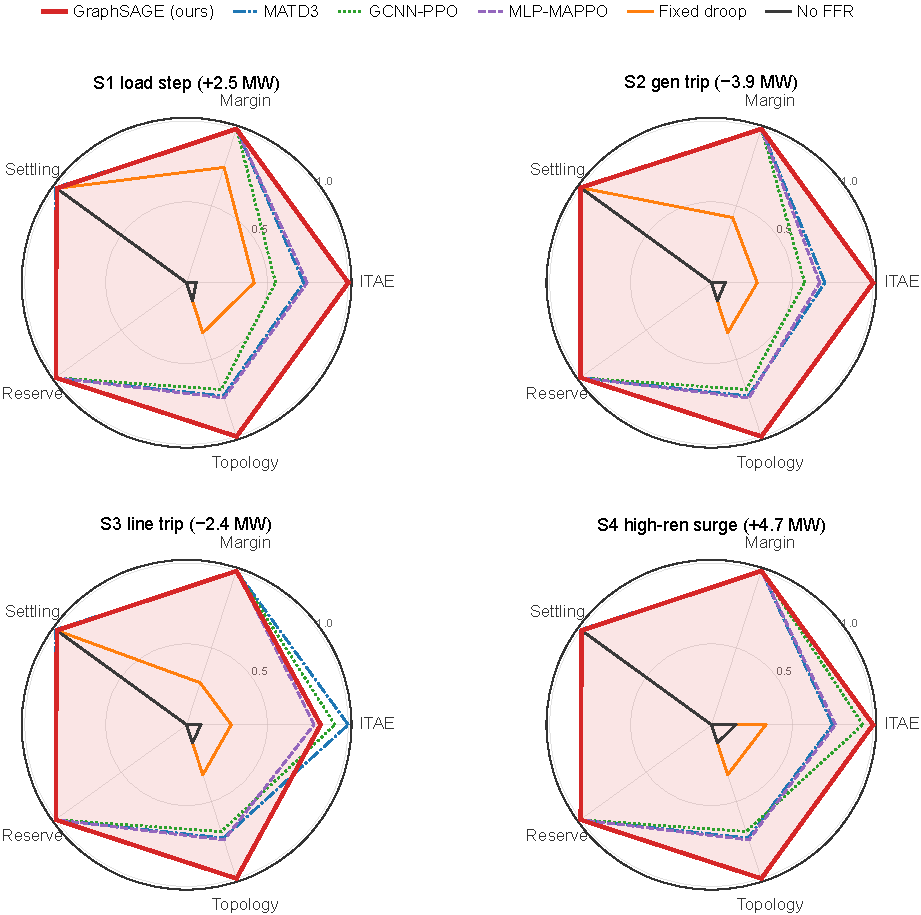
\includegraphics[width=0.98\textwidth]{img/fig1_radar.pdf}
\caption{Per-scenario performance radar over five axes post-event IAE, frequency margin, settling speed, reserve delivery, and topology robustness each oriented so larger is better and normalized by the best in-group value (outer ring). The topology axis is system-level, hence identical across panels.}
\label{fig:radar_overview}
\end{figure*}
 
% ==================================================================
\subsection{Frequency-Security Performance}
\label{ssec:res_stability}
% ==================================================================
 
Fig.~\ref{fig:freq_grid} overlays the mean frequency trajectories of the six controllers for the four contingencies ($\pm1\sigma$ band shown for the proposed controller).

\begin{figure}[!h]
\centering

\includegraphics[width=0.95\linewidth]{section1_stability/fig_freq_grid.pdf}
\caption{Frequency response (mean; $\pm 1\sigma$ band on the proposed controller; $0.05$~s sub-step traces, Sec.~S-VII). Red: UFLS-1 ($49.0$~Hz); orange: $49.5/50.5$~Hz alarm; green band: $\pm50$~mHz settling (ENTSO-E standard frequency range).}
\label{fig:freq_grid}
\end{figure}
 
\emph{Frequency excursion.}
The shared safety envelope holds the post-event nadir at the $49.5$~Hz alarm for all four learning controllers in S1--S3 and caps the over-frequency zenith at $50.5$~Hz in S4, so each achieves a unit FFR-success rate. The two non-learning controls breach the alarm: fixed droop reaches $48.75$~Hz on the severe generation trip~S2 and $51.51$~Hz on the surge~S4, and no-FFR $48.42$ and $51.91$~Hz, both with zero FFR success. Relative to fixed droop the proposed controller therefore raises the S2 nadir by $0.75$~Hz and cuts the S4 over-frequency excursion above nominal from $1.51$~Hz to $0.50$~Hz. The sawtooth visible on the proposed trace at the band edge is the closed-form nadir projection activating step-by-step, resolved by the $0.05$~s sub-step trace.

\emph{Integral error and settling.}
Among the safe controllers the discriminators are the integral error and the settling speed. On the windowed IAE$_{\mathrm{post}}$ \eqref{eq:iae_post} the saturating MATD3 attains the smallest in-window error in every scenario ($2.65$--$5.30$~Hz$\cdot$s) by holding near-maximum effort throughout the window; the proposed controller follows within $7$--$15$\,\% ($2.83$--$5.76$) and is $18$--$21$\,\% below fixed droop ($38$--$50$\,\% below no-FFR) while keeping the nadir safe. This windowed metric, however, rewards exactly the sustained saturation that the unwindowed metrics expose as pathological. The latter are decisive: the proposed controller has the lowest IAE$_{\mathrm{tot}}$ in all four scenarios ($3.7$--$6.6$ vs.\ $7.5$--$45.7$) and an ITAE of $9.3$--$34.1$ against $671$--$5317$ for the other learning controllers a $20$--$72\times$ reduction relative to the best of them because it re-enters the $\pm50$~mHz settling band (Table~\ref{tab:fsec_standards}) in $9$--$14$~s, $1.9$--$3.0\times$ faster than the next-best learning controller ($17$--$43$~s), and \emph{stays} there, whereas MATD3 and GCNN-PPO sustain a high-amplitude oscillation that the $50$-s window of IAE$_{\mathrm{post}}$ does not penalize. Fixed droop settles comparably fast only by leaving the nadir below the alarm. The run-to-run spread on the training feeder is the smallest of all controllers (standard deviation of IAE$_{\mathrm{post}}\le0.002$~Hz$\cdot$s, against $0.06$--$0.70$ for the other learning methods), so the reported means are not seed artifacts.

\emph{FFR-success and RoCoF.}
The FFR-success column cleanly separates the learning controllers (unit success nadir held within the alarm band) from the non-learning controls (zero). The maximum RoCoF is $\approx0.5$~Hz/s for every learning controller and below $1.3$~Hz/s throughout, well inside the IEEE Std~1547 $2.0$~Hz/s ride-through; consistent with Section~\ref{sec:method:safety}, peak RoCoF is set by the backbone inertia rather than by the GFL action and so does not discriminate the controllers.

\begin{figure}[!t]
\centering
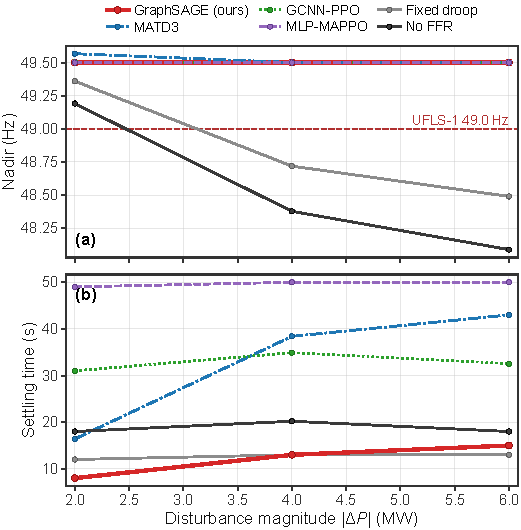
\includegraphics[width=0.92\columnwidth]{img/fig_severity.pdf}
\caption{Severity scaling ($2$--$6$~MW): (a) nadir and (b) settling time.}
\label{fig:severity}
\end{figure}

\emph{Severity scaling.}
Sweeping the imbalance from $2$ to $6$~MW ($13$--$38$\,\% of $S_{\mathrm{base}}$, Fig.~\ref{fig:severity}), every learning controller holds the nadir at $49.5$~Hz while the non-learning controls fall to $48.49/48.09$~Hz, so the proposed controller's nadir margin over fixed droop widens from $0.14$ to $1.01$~Hz. Among the safe controllers it settles in $8$--$15$~s against $16$--$50$~s, degrading by only $7$~s over the sweep where MATD3 degrades by $27$~s ($16\!\to\!43$~s) gracefully rather than as a cliff.
 
% ==================================================================
\subsection{Topology Generalization}
\label{ssec:res_topo}
% ==================================================================
 
Topology generalization the central claim is shown by the training-to-unseen retention over the $24$-reconfiguration hold-out (Fig.~\ref{fig:topo_gap}) and by the spread of post-event IAE across those unseen topologies (Fig.~\ref{fig:unseen}).

\begin{figure}[!t]
\centering
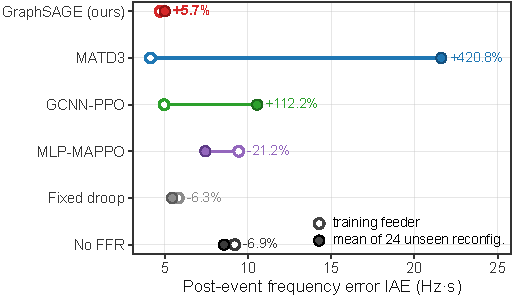
\includegraphics[width=0.92\columnwidth]{img/fig_topology.pdf}
\caption{Train-to-unseen IAE over the $24$-reconfiguration hold-out (open: training $G_0$; filled: unseen mean; label: gap).}
\label{fig:topo_gap}
\end{figure}

\emph{Base-to-unseen retention.}
The proposed controller carries its training-feeder IAE$_{\mathrm{post}}$ of $4.74$~Hz$\cdot$s to $5.01$ on the unseen reconfigurations (gap $+5.7$\,\%, retention $0.946$) the lowest unseen error of any controller, $53$\,\% below the next-best learning controller (GCNN-PPO, $10.56$). The fixed-adjacency and non-graph baselines collapse despite near-identical training-feeder performance: GCNN-PPO degrades by $+112$\,\% ($4.98\!\to\!10.56$) and MATD3 by $+421$\,\% ($4.15\!\to\!21.6$). MLP-MAPPO shows a \emph{negative} gap ($-21$\,\%) only because its training-feeder error is already $2\times$ ours ($9.45$~Hz$\cdot$s) a floor effect, not generalization; the same artifact explains the small gaps of the non-responsive classical references. The inductive encoder supplies not only the lower error but its predictability: the across-topology standard deviation is $0.17$~Hz$\cdot$s, against $4.68$ (GCNN-PPO, $27\times$), $6.69$ (MATD3, $38\times$), and $1.13$ (MLP-MAPPO, $6\times$).

\begin{figure}[!h]
\centering
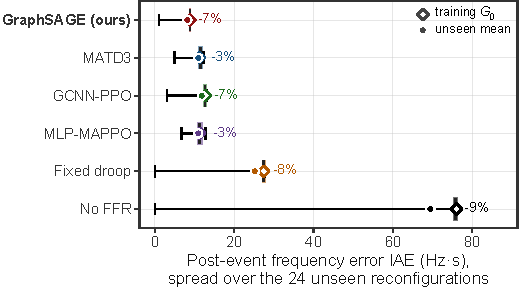
\includegraphics[width=0.95\columnwidth]{img/fig_unseen_iae.pdf}
\caption{Post-event IAE across the $24$ unseen reconfigurations (box: IQR; whiskers: min--max; diamond: training $G_0$).}
\label{fig:unseen}
\end{figure}

\emph{Across the hold-out.}
Across the $24$ unseen topologies the proposed controller's IAE stays within a $\pm0.17$~Hz$\cdot$s band of its training value and remains below the next-best controller on the hold-out fixed droop, which trades its low IAE for a breached nadir with high significance (paired Wilcoxon signed-rank, $p<10^{-6}$); every learning baseline is dominated on \emph{every} topology. MATD3 and GCNN-PPO spread widely (unseen IAE up to $\approx24$ and $19$~Hz$\cdot$s). The tight, low cluster in Fig.~\ref{fig:unseen} is the visual signature of an inductive encoder that re-aggregates over each active edge set instead of reusing a fixed adjacency, and it persists in operation: on the unseen topologies the proposed controller still settles in $16.5$~s on average, against $37$--$49.5$~s for the learning baselines.
 
% ==================================================================
\subsection{Economic Efficiency}
\label{ssec:res_econ}
% ==================================================================
 
This subsection evaluates the controller as a \emph{price taker} against the DLMP and reserve prices set in the upper layers (Section~\ref{sec:model:layers}), reporting the per-event DSO settlement each controller induces under a common price deck \cite{rahimiyan2016pricetaker,li2014dlmp}. Each event is settled as
\begin{equation}
  C_{\mathrm{event}}
   = \lambda_{\mathrm{cap}}\,R_{\mathrm{armed}}\,T_{\mathrm{ev}}
   + \lambda_{\mathrm{act}}\,E_{\mathrm{ffr}}
   + \mathrm{VOLL}\cdot E_{\mathrm{shed}},
  \label{eq:dso_cost}
\end{equation}
where $R_{\mathrm{armed}}=K_{\mathrm{peak}}\,\delta$ is the reserve armed at the band edge, $E_{\mathrm{ffr}}$ the delivered FFR energy, and $E_{\mathrm{shed}}$ the energy-not-served of a staged ENTSO-E UFLS model ($5/15/30\,\%$ of load below $49.0/48.5/48.0$~Hz) applied to the realized trajectory. Prices follow the reserve-context convention: $\lambda_{\mathrm{cap}}=50$~\texteuro/MW/h, $\lambda_{\mathrm{act}}=100$~\texteuro/MWh, $\mathrm{VOLL}=3000$~\texteuro/MWh, with a $\{1500,8000\}$~\texteuro/MWh VOLL sweep confirming ranking invariance (Sec.~S-VII).

\begin{figure}[!t]
\centering
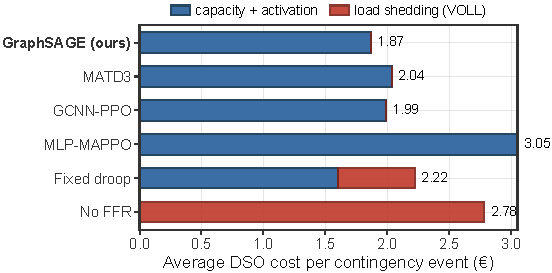
\includegraphics[width=0.95\columnwidth]{img/fig_pareto.pdf}
\caption{Average per-event DSO settlement \eqref{eq:dso_cost}: service payments (capacity + activation) vs.\ load-shedding penalty (VOLL).}
\label{fig:pareto}
\end{figure}

\emph{Avoided shedding and cost stability.}
The decisive economic split is delivery (Fig.~\ref{fig:pareto}): on the severe generation trip (S2) the non-learning controls fail to arrest the swing and incur per-event settlements of $9.89$~\texteuro\ (No-FFR, dominated by VOLL load-shedding cost) and $4.02$~\texteuro\ (Fixed Droop, partial shedding), whereas all four learning controllers eliminate shedding entirely and pay only for reserve. Among learning controllers the proposed method is the most economical ($1.73$--$1.78$~\texteuro\ across S1--S4, tightest scenario spread) versus ${\approx}1.98$~\texteuro\ for GCNN-PPO, $1.98$--$2.02$~\texteuro\ for MATD3, and $2.71$~\texteuro\ for MLP-MAPPO. MLP-MAPPO incurs the highest reserve bill in the group---a constant commitment regardless of scenario severity---consistent with its larger static dispatch that yields weaker settling. The proposed controller thus pairs the lowest per-event cost among learning methods with the best frequency-security and topology-robustness outcomes.
 
% ==================================================================
\subsection{Discussion}
\label{ssec:discussion}
% ==================================================================
 
Taken together, the studies separate two control philosophies that the windowed IAE$_{\mathrm{post}}$ alone cannot. MATD3 converges to a near-saturated, state-insensitive commitment its actions ride the actuator limits regardless of operating point which buys the smallest in-window error on the under-frequency events but at a characteristic cost signature: a slow, high-amplitude post-event swing (ITAE $\sim\!10^3$), a ${\approx}2.0$~\texteuro\ reserve bill second only to MLP-MAPPO ($2.71$~\texteuro), and a $+421$\,\% collapse on unseen topologies. The proposed controller commits reserve \emph{selectively}: the inductive GraphSAGE encoder learns topology-invariant bus features and re-aggregates over whatever feeder is active, so the policy delivers the lowest total and time-weighted error, settles $1.9$--$3.0\times$ faster and stays settled, holds a scenario-invariant DSO cost, and carries its performance across reconfigurations with a $0.17$~Hz$\cdot$s spread. The encoder-only ablation, identical but for the encoder, loses both the low error and more tellingly its cross-topology predictability, which attributes the gain to the inductive graph representation rather than to the cooperative RL stack.

The principal limitation is one of validation level. The frequency model is small-signal: it captures reconfiguration through the Kron-reduced Jacobian but omits electromagnetic-transient (EMT) converter behavior and the inner voltage/current loops, and the closed loop is exercised without communication delay or measurement noise. Validation on a commercial EMT platform (e.g., PSCAD or EMTP-RV) and in a hardware-in-the-loop testbed is therefore the principal next step.




\section{Conclusion} \label{sec:conclusion}
This paper replaced the classical droop loop for fast frequency response in $100$\,\% inverter-based islanded microgrids with a topology-adaptive cooperative MARL controller: an inductive GraphSAGE encoder over the active feeder graph feeds a parameter-shared MAPPO actor whose per-DER action jointly sets a power reference and a local droop gain, inside a shared safe-by-construction envelope. Trained on a single feeder topology and evaluated zero-shot on $24$ unseen reconfigurations of a modified islanded IEEE 123-bus feeder, every learning controller stayed nadir-safe, but the proposed controller settled $1.9$--$3.0\times$ faster with a $20$--$72\times$ lower time-weighted error, and retained its post-event integral frequency error within $6\%$ of the training-feeder value the lowest unseen error of any controller, against $+112$ to $+421\%$ degradation for fixed-adjacency and saturating baselines at the lowest per-event cost among the learning controllers. An encoder-only ablation attributed this cross-topology predictability to the inductive graph representation rather than the cooperative RL stack; inductive graph encoders are thus a practical route to FFR controllers that remain effective as feeders are reconfigured, without retraining. Validation on a commercial electromagnetic-transient platform and a hardware-in-the-loop testbed under realistic communication delay and measurement noise is the principal next step.





% \section*{Acknowledgments}
% The authors would like to acknowledge the support provided by VinUniversity.



% {\appendix[Proof of the Zonklar Equations]
% Use $\backslash${\tt{appendix}} if you have a single appendix:
% Do not use $\backslash${\tt{section}} anymore after $\backslash${\tt{appendix}}, only $\backslash${\tt{section*}}.
% If you have multiple appendixes use $\backslash${\tt{appendices}} then use $\backslash${\tt{section}} to start each appendix.
% You must declare a $\backslash${\tt{section}} before using any $\backslash${\tt{subsection}} or using $\backslash${\tt{label}} ($\backslash${\tt{appendices}} by itself
%  starts a section numbered zero.)}



% %{\appendices
% %\section*{Proof of the First Zonklar Equation}
% %Appendix one text goes here.
% % You can choose not to have a title for an appendix if you want by leaving the argument blank
% %\section*{Proof of the Second Zonklar Equation}
% %Appendix two text goes here.}



% \section{References Section}
% You can use a bibliography generated by BibTeX as a .bbl file.
%  BibTeX documentation can be easily obtained at:
%  http://mirror.ctan.org/biblio/bibtex/contrib/doc/
%  The IEEEtran BibTeX style support page is:
%  http://www.michaelshell.org/tex/ieeetran/bibtex/
 
%  % argument is your BibTeX string definitions and bibliography database(s)
% %\bibliography{IEEEabrv,../bib/paper}
% %
% \section{Simple References}
% You can manually copy in the resultant .bbl file and set second argument of $\backslash${\tt{begin}} to the number of references
%  (used to reserve space for the reference number labels box).


\bibliographystyle{IEEEtran}
\bibliography{Ref}

\vfill

\end{document}